% !TeX root = ../../../thesis.tex

\section{Simulation}
\label{sec:simulation-evaluation}

The evaluation with actual hardware has now been done.
With that evaluation the continuous transmission method was used for each LED as detailed in \autoref{subsec:continuous-method-modulation}.
This means that every LED was continuously transmitted its ID.
The software simulation that will be done in this chapter, will use the probabilistic method as explained in \autoref{subsec:probabilistic-method-modulation}.
Both of the interference solutions will then have been used to evaluate the system.




Before the actual simulation itself, the parameters of the probabilistic approach such as $\epsilon$ need to be set.
$1 - \epsilon$ is the probability that for every point in time the number of LEDs that are modulating will not exceed $m$, as discussed in \autoref{subsec:probabilistic-method-modulation}.
This will determine if interference can occur and therefor this will determine the accuracy of the system.

For the rest of this simulation a Gold sequence set with a LFSR length of $n = 7$ will be used.
The codes in this set have length $L = 2^n - 1 = 127$ and $N = 2^n + 1 = 129$ unique Gold sequences.
So all the IDs that are assigned to the LEDs have length 127 and there will be 129 unique LEDs.

This simulation does the following: 

\begin{itemize}

	\item For the error $\epsilon$ the probability $p$ and the time to complete the $k$ slots are calculated (See \autoref{subsec:probabilistic-method-modulation}).

	\item At each time slot, each LED will use the probability $p$ to determine if it will transmit its ID.

	\item If a certain LED transmits its ID, the ID is added to a signal vector which represents the current draw in the hardware testbeds.

	\item When the entire signal has been constructed, the decoding process begins. All 129 IDs are used to decode the incoming signal for every time slot.

	\item During the decoding, the results are analyzed and together with the information that is known when a particular LED transmitted at what time, the results are classified into four categories: true-positive, true-negative, false-positive and false-negative. This is done for each time slot.

	\item With those four categories, the precision, recall and the F-measure are calculated.



\end{itemize}




Let's set $\epsilon = 0.1$, meaning that the probability that there will be less than or equal to $m$ LEDs modulating for every point in time will be 0.9 or 90 \%, where $m$ is the maximum number of simultaneous transmitters such that no destructive interference takes place.
Now that the simulation steps have been explained and all variables have been set, the simulation itself is performed. 

\begin{figure}[ht]
	\centering
	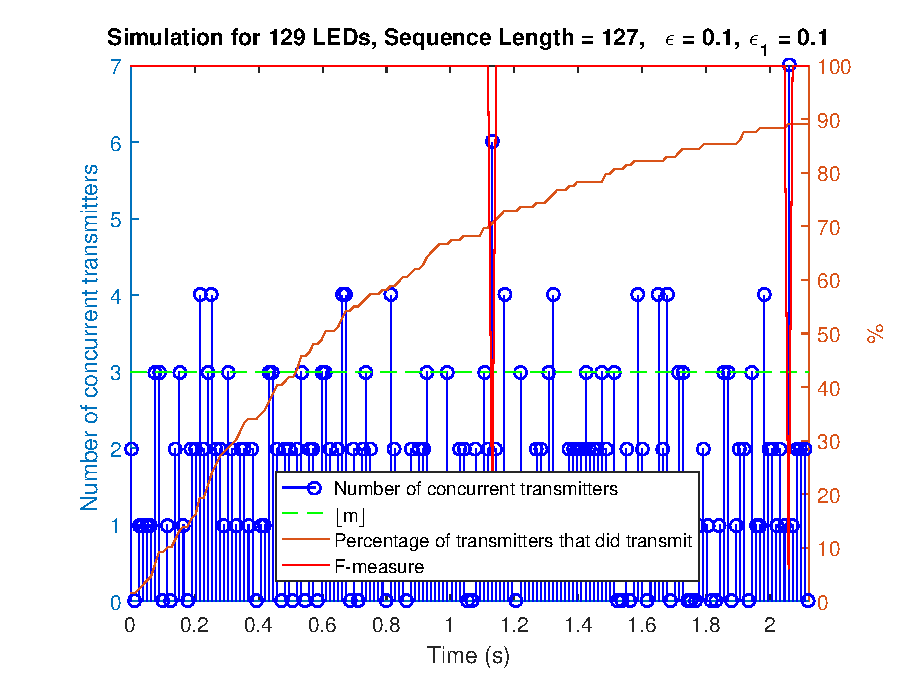
\includegraphics[width=\textwidth]{chapters/evaluation-chapters/simulation/sim-concurrent-tx-and-f-measure-eps=1-n=7.eps}
	\caption{Results of the simulation with $\epsilon = 0.1$. Figure shows the number of concurrent transmitters at each point in time along with $m$ and the percentage of transmitters that have transmitted. Also the F-measure is shown.}
	\label{fig:sim-concurrent-tx-and-f-measure-eps=1-n=7}
\end{figure}



The results of the simulation can be seen in \autoref{fig:sim-concurrent-tx-and-f-measure-eps=1-n=7}.
In this figure the number of concurrent transmitters over time are represented by the blue dots and the left y-axis.
The maximum number of simultaneous transmitters such that no destructive interference takes place, $m$, is represented with the green dashed line.
When the number of concurrent transmitters is below or equal to the $m$-line, it is guaranteed that no interference will occur, as proven in \autoref{sec:interference-solution}.
But when the number of concurrent transmitters is above the $m$-line, it may not be possible to successfully decode the signal
This depends on what the cross-correlation with the other IDs is, if they cancel each other out or if they enhance each other.

In \autoref{fig:sim-concurrent-tx-and-f-measure-eps=1-n=7} the F-measure is represented by the red line.
At each point in time the correlation calculations are performed for all the 129 IDs.
All the true-positives, true-negatives, false-positives and false-negatives are used to calculate the F-measure according to \autoref{eq:F-measure}.
The results are then plotted in the figure.
In \autoref{fig:sim-concurrent-tx-and-f-measure-eps=1-n=7}, it can be seen that whenever the number of concurrent transmitters is below the $m$-line, the F-measure is equal to 1.
For example, from time 0 s until 0.25 s, the number of concurrent LEDs transmitting their IDs never exceed the $m$-line and as a result the F-measure remains at 1 during this time.
This means that everything in the decoding process went well, there were no false-positives and/or false-negatives.

When the number of concurrent transmitters is above the $m$-line, two things can happen: either there is enough interference to cause false-positives and/or false-negatives, or there is not enough interference and everything will go well.
An example of the latter case: From 0.6 s until the end, the number of concurrent LEDs which are transmitting their IDs goes above the $m$-line four times but the F-measure stays 1 during this window.
This is an example that the interference created by these IDs is not high enough to cause problems when decoding.
Examples for when the interference is too high to successfully decode the data can be seen at the following times in the \autoref{fig:sim-concurrent-tx-and-f-measure-eps=1-n=7}: 0.27 s, 0.4 s, 0.55 s and 0.6 s.
At each of these timestamps the number of concurrent LEDs which are transmitting their IDs is so high that they cause so much interference that there are problems with the decoding.
And as a result the F-measure has significant drops at each of those timestamps.
For example at time 0.4 s there were 31 false-positives and 0 false-negatives.



In \autoref{fig:sim-concurrent-tx-and-f-measure-eps=1-n=7} the percentage of transmitters that have transmitted can also be seen, by looking at the orange line.
This line is approximately a linear line due to each LED has a limited amount of slots to transmit and each slot has the same probability of being chosen so the number of transmitters that are transmitting is approximately uniformly divided.


The percentage that the number of concurrent LEDs is above $m$ is roughly equal to 12 \%.
This number will get closer and closer to $\epsilon$ the longer the simulation takes.


This simulation has been performed more than ten times.
Each run was slightly different due to the probabilistic approach.
But every time similar results could be seen concerning the accuracy and the total time taken.
The total time that the simulation takes is roughly 1 s.
The time corresponds with the theoretical time calculated in \autoref{subsec:probabilistic-method-modulation} as can be seen in \autoref{tbl:probabilistic-method-time-as-function-N}.
So this was a fast time but multiple errors occurred as can be seen from the drops in the f-measure.



\begin{figure}[ht]
	\centering
	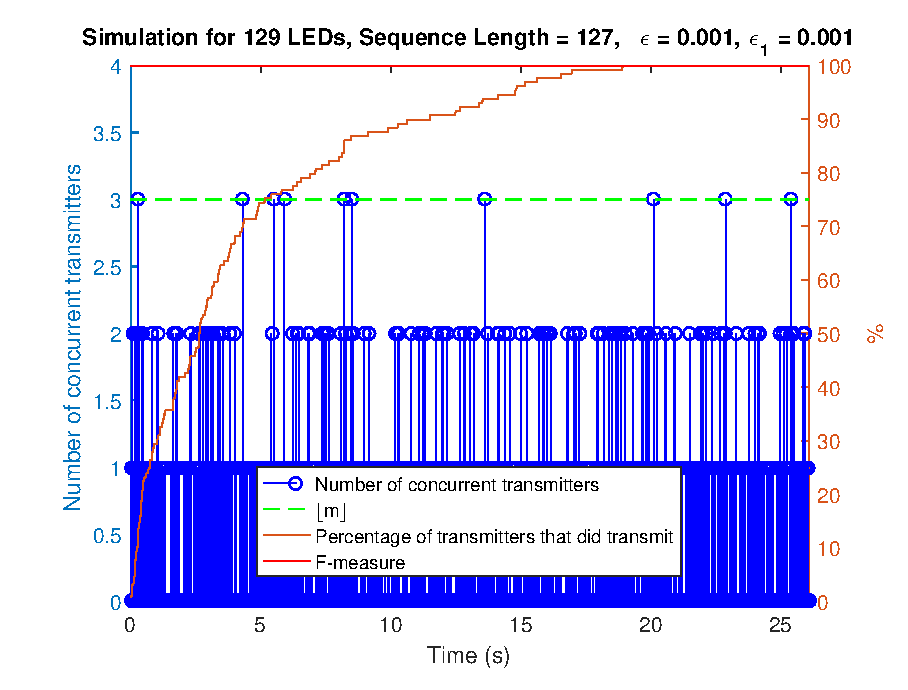
\includegraphics[width=\textwidth]{chapters/evaluation-chapters/simulation/sim-concurrent-tx-and-f-measure-eps=001-n=7.eps}
	\caption{Results of the simulation with $\epsilon = 0.001$. Figure shows the number of concurrent transmitters at each point in time along with $m$ and the percentage of transmitters that have transmitted. Also the F-measure is shown.}
	\label{fig:sim-concurrent-tx-and-f-measure-eps=001-n=7}
\end{figure}






The same simulation is done again, but now with $\epsilon = 0.001$.
The plots can be seen in \autoref{fig:sim-concurrent-tx-and-f-measure-eps=001-n=7} which show the same kind of information as in the simulation figure shown before.
This simulation with the new value for $\epsilon$ has also been performed more than ten times.
The distribution of the number of concurrent LEDs was slightly different each time but the F-measure was always the same.
At no time the number of concurrent LEDs goes above the $m$-line, so there will be no interference as can also be seen by looking at the F-measure which is a constant 1.
So with $\epsilon = 0.001$ it is an accurate setup that can use all the IDs that are provided by the LFSR to construct the Gold sequences.
But the simulation takes roughly 4 s.
The time corresponds with the theoretical time calculated in \autoref{subsec:probabilistic-method-modulation} as can be seen in \autoref{tbl:probabilistic-method-time-as-function-N}.
This is still a relative small amount of time, but still 4 times larger than the previous simulation.
This simulation represents a slow but accurate result.



 

These simulations show that for the probabilistic method there is a clear trade off between time and accuracy.
For a given set of IDs, a low value for $\epsilon$ gives high accuracy but the also the a high time.
A high value for $\epsilon$ gives lower accuracy but the also the time becomes smaller.